\documentclass[a4paper,12pt]{article}
\usepackage{graphicx}
\usepackage{rotating}
%\usepackage{bbding}
\begin{document}

\title{System Validation Project Report}
\author{
	Suryansh Sharma \\ 
	\texttt{S.sharma-13@student.tudelft.nl}
 	\and 
	Snehal Jauhri \\
	\texttt{S.jauhri@student.tudelft.nl} 
	\and
	Suhail Nogd \\
	\texttt{S.T.S.nogd@student.tudelft.nl} 	
	 \and 
	Apoorva Arora\\
	\texttt{A.Arora-1@student.tudelft.nl} 
}

\date {\today}
\maketitle

\section{Introduction}
This is a project done as part of TU Delft's IN4387 System Validation course. The project concerns designing, modelling and validating a controller for a Transfer system in an Industrial Silicon Wafer production plant.
The system consists of a UV Lamp that projects a design onto a wafer inside a vacuum chamber. The wafers are transferred to the Lamp via two Airlocks. The wafers are handled by robots from their initial position on Input stacks to their final position on Output stacks. The wafers move along the production line from their Initial state (on the Input Stacks), are printed on by the Lamp and reach the Final state (on the Output stacks).

\section{Requirements}

\subsection{System Components}
The system consists of the following physical components:
\begin{itemize}
\item Lamp/Projector: L
\item Inner Doors: DI1, DI2
\item Outer Doors: DO1, DO2
\item Input Stacks: I1, I2
\item Output Stacks: O1, O2
\item Airlocks: A1, A2
\item Outer Robots: R1, R2
\item Inner Robot: R3
\end{itemize}

\subsection{Functional Requirements}
\subsubsection{Overall requirements of the System:}
\begin{itemize}
\item As long as the Output Stacks are not full, wafers keep moving along the production line. (System is deadlock free) \textbf{(Safety)}
\item Both the Inner and Outer Doors of an Airlock must NOT be open at the same time.\textbf{ (Safety)}
\item Doors must not be closed while the robot is picking up/placing a wafer in the Airlock\textbf{ (Safety)}
%\item Doors must not get stuck\textbf{(Safety)}
%\item Robots must not stop before reaching their destinations\textbf{ (Safety)}
\end{itemize}

\subsubsection{System Component Requirements:}
These are the individual component requirements:
\begin{enumerate}
%\item Lamp L
	%\begin{itemize}
	%\item The Lamp should be undisturbed during printing.\textbf{ (Safety)}
	%\item The Lamp will turn off after completion of printing.	
	%\end{itemize}
\item Doors: DI1, DI2, DO1, DO2
	\begin{itemize}
	\item Inner and Outer Doors  (DIx, DOx) of an Airclock (Ax) should never be open at the same time. (Vaccuum must be preserved) \textbf{ (Safety)}
	\item Inner Door (DIx) should be opened ONLY if it's corresponding Outer Door (DOx) is closed and vice versa. \textbf{ (Safety)}
	\end{itemize}

\item Output Stacks: O1, O2
	\begin{itemize}
	\item Wafer should not be put on a full Output Stack.\textbf{ (Safety)}
	\end{itemize}

\item Outer Robots: R1, R2
	\begin{itemize}
	%\item The Outer Robots will pick up a wafer from its corresponding Input stack.
	%\item The Outer Robots will place the Input wafer on its corresponding Airlock.
	%\item The Outer Robots will pick up a finished wafer from its corresponding Airlock.
	%\item The Outer Robots will place the finished wafer on its corresponding Output stack.
	\item The Outer Robot (Rx) should pick the next Input wafer ONLY after delivering a finished wafer to it's corresponding Output Stack (Ox).\textbf{ (Safety)}
	\end{itemize}

\item Inner Robot: R3
	\begin{itemize}
	%\item The Inner Robot will pick up a detected Input wafer from an Airlock.
	\item The Inner Robot should place the Input wafer on the Lamp ONLY when the Lamp's stack is empty.\textbf{ (Safety)}
	%\item The Inner Robot will pick up a finished wafer from the Lamp.
	%\item The Inner Robot will place the finished wafer on its corresponding Airlock.
	\item The Inner Robot should pick the next Input wafer ONLY after delivering a finished wafer to it's corresponding Airlock (Ax).\textbf{ (Safety)}
	\end{itemize}

\end{enumerate}
%Extension: A Robot can use 2 hands independently and having separate control -- one for Finished and one for New

% Maybe need this Later
\iffalse
\subsection{Sequence}
Initial Conditions: All Doors are closed. Lamp is off. Robots R1 and R2 are near the Input Stacks. Robot R3 waits at Lamp. Airlocks A1, A2 are closed. Input Stacks are not empty and Output Stacks are not full.
\subsubsection {I/O Retrieval Sequence }
\begin{itemize}
\item Check if Ix Stack not empty
\item Robot Rx moves to Ix
\item Robot Rx picks up the wafer at Ix 
\item Open the Outer Door DOx
\item Move to DOx
\item Place wafer at Ax
\item Close DOx
\item Wait till DOx opens
\item Check if Ox Stack not full
\item Pick (finished)wafer from Ax
\item Close DOx
\item Move to Ox
\item Place (finished)wafer at Ox
\item GOTO 1
\end{itemize}

\subsubsection {Printing Sequence}
\begin{itemize}
\item Detect wafer at Ax
\item Check if DOx is closed
\item Open DIx
\item R3 moves to DIx
\item Pick wafer at Ax
\item Close DIx
\item Robot R3 places wafer on Lamp L
\item Lamp L turns on
\item Detect completed wafer on Lamp L [Assumption: Lamp has turned off]
\item Check if DOx is closed
\item Open DIx
\item R3 moves to DIx
\item Place wafer at Ax
\item Close DIx
\item Open DOx
\item GOTO 1
\end{itemize}
\subsection{System Requirements}
These are the individual component's constraints:
\begin{enumerate}
\item Lamp L
	\begin{itemize}
	\item The Lamp should be undisturbed during printing.
	\item The Lamp will be turned off after completion of printing.	
	\end{itemize}
\item Inner Doors: DI1, DI2
	\begin{itemize}
	\item The Inner Doors may be opened only if the Outer Doors are closed.
	\end{itemize}

\item Outer Doors: DO1, DO2 
	\begin{itemize}
	\item The Outer Doors may be opened only if the Inner Doors are closed.
	\end{itemize}

\item Output Stacks: O1, O2
	\begin{itemize}
	\item No Wafer shall be put on a full Output Stack.  
	\end{itemize}

\item Outer Robots: R1, R2
	\begin{itemize}
	\item The Outer Robots will pick up a wafer from its corresponding Input stack.
	\item The Outer Robots will place the Input wafer on its corresponding Airlock.
	\item The Outer Robots will pick up a finished wafer from its corresponding Airlock.
	\item The Outer Robots will place the finished wafer on its corresponding Output stack.
	\item The Outer Robots will pickup the next Input wafer only after delivering a finished wafer to it's corresponding Output Stack.
	\end{itemize}

\item Inner Robot: R3
	\begin{itemize}
	\item The Inner Robot will pick up a detected Input wafer from an Airlock.
	\item The Inner Robot will place the Input wafer on the Lamp only when it is empty
	\item The Inner Robot will pick up a finished wafer from the Lamp.
	\item The Inner Robot will place the finished wafer on its corresponding Airlock.
	\item The Inner Robot will pickup the next Input wafer only after delivering a finished wafer to it's corresponding Airlock.
	\end{itemize}

\end{enumerate}
\fi

\section{Interactions} 
\subsection {Commands to Actuators}
The following are the commands given by the controller to the actuators of the system. The meaning can be interpreted as: \bigskip

\textbf{Command( Target actuator, optional parameters)}
\begin{itemize}
\item MoveTo(x, D) [x: R1, R2, R3 ; D: Lamp, Airlocks, Input/Output Stacks]		Move to assigned destination.	
\item PickupWafer(x, D)															[x: R1, R2, R3 ; D: Lamp, Airlocks, Input Stacks] 					Picks up the wafer.
\item PlaceWafer(x, D) 															[x: R1, R2, R3 ; D: Lamp, Airlocks, Output Stacks]					Places the wafer.
\item OpenDoor(x,s) 																[x: DI1, DI2, DO1, DO2; s:Open, Close]  														Opens the corresponding door.
\item CloseDoor(x) 																[x: DI1, DI2, DO1, DO2]														Closes the corresponding door.
\end{itemize}
The commands are valid for the combinations of target Actuators and Destinations shown below:
\begin{table}[!h]
\centering
{%
\begin{tabular}{l|l|l|l|l|l|l|l|}
\cline{2-8}
                         & Lamp & Airlock1 & Airlock2 & Input1 & Input2 & Output1 & Output2 \\ \hline
\multicolumn{1}{|l|}{Robot1} &   &   & Y   & Y  &    & Y  &    \\ \hline
\multicolumn{1}{|l|}{Robot2} &   &    & Y  &    & Y  &    & Y  \\ \hline
\multicolumn{1}{|l|}{Robot3} & Y & Y  & Y  &    &    &    &    \\ \hline
\end{tabular}%
}
\end{table}
\subsection {Reading Sensors}
The following are the commands used by the controller to read the data provided by the sensors of the system. The meaning can be interpreted as: \bigskip

\textbf{Command(Target sensor, Return Value by sensor)}
\begin{itemize}
\item CheckInputStack(x, s)              [x: I1,I2 ; s: Present, Absent] 
\item CheckOutputStack(x, s)          [x: O1,O2 ; s: Full, Empty]
\item CheckLamp(L, s)	                  [L: Lamp ; s: Busy, CompletedPrinting]	
\item CheckAirlock(x, s)                    [x: A1,A2 ; s : WaferPresent, WaferAbsent]  % if wafer present close outer door, open inner door;  else inner door remains closed, and outer remains open?? optimisation?? 
\end{itemize}
\newpage
\section{Architecture}
\begin{figure}[ht]
\centering
    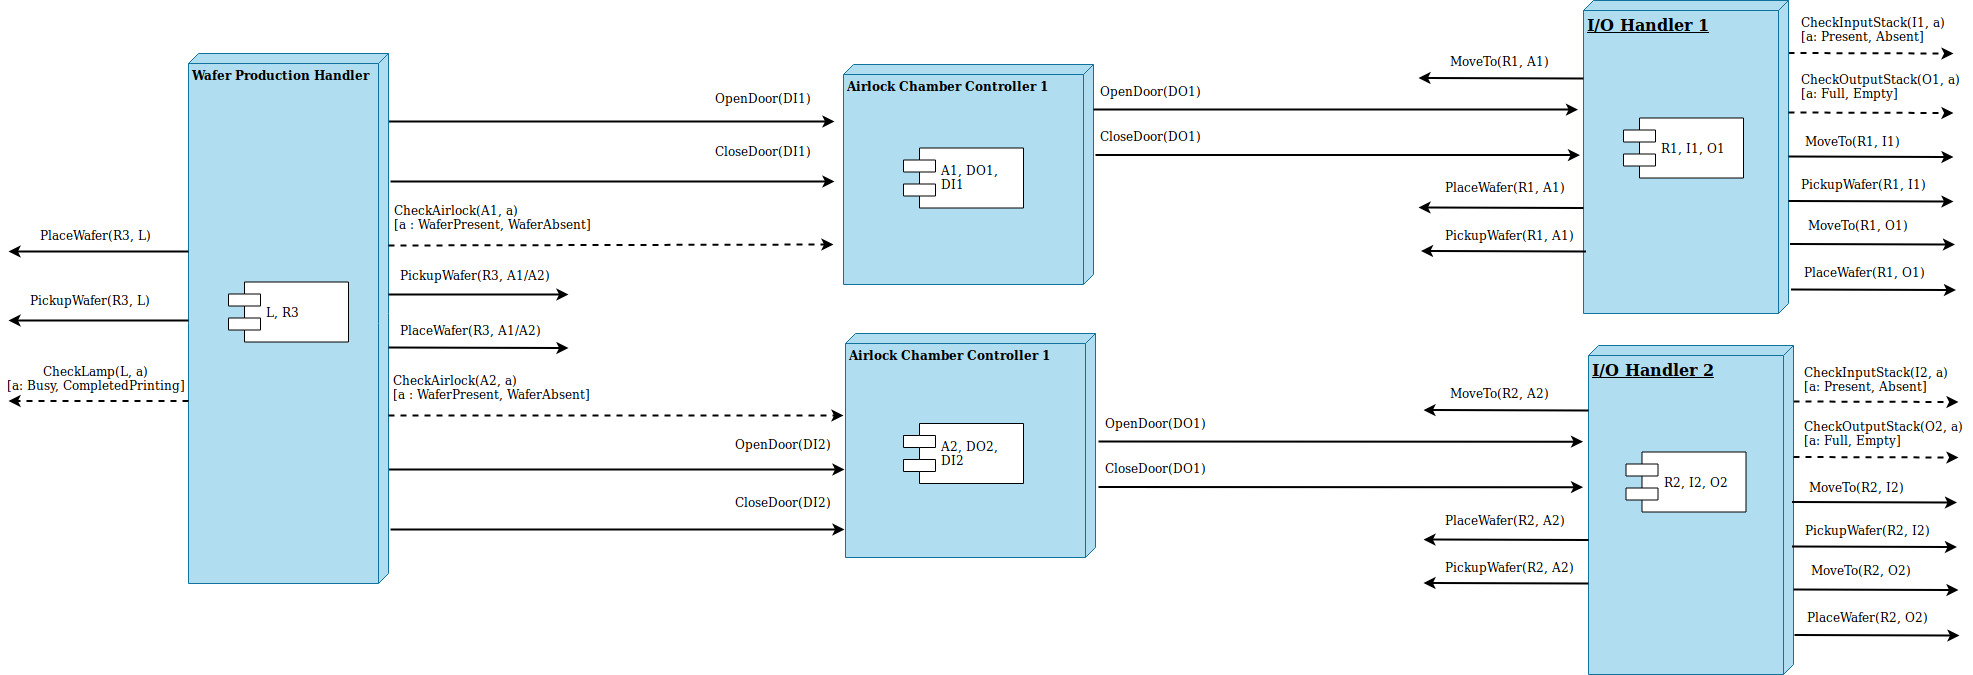
\includegraphics[angle=90, width=15cm,height=20cm]{Architecture.jpg}
  \caption{Architecture Diagram of System}
  \label{fig:arch1}
\end{figure}
Figure \ref{fig:arch1} shows the Architecture of the system described above with five parallel controllers along with the various entities (Sensors and Actuators) they control.

\end{document}
